
\documentclass{article}
\usepackage{amsmath}
\usepackage{listings}
\usepackage{graphicx}
\usepackage[margin=1in]{geometry}
\usepackage{hyperref}
\pagenumbering{gobble}
\setlength{\tabcolsep}{10pt}
\renewcommand{\arraystretch}{1.7}
 
\begin{document}

\section*{\hfil H. Kotak Cokelat\hfil}

% \begin{center}
% \begin{tabular}{ |cc| } 
%  \hline
%  Time Limit & 2 detik \\
%  \hline 
%  Memory Limit & 256 MB \\
%  \hline
% \end{tabular}
% \end{center}

\subsection*{Deskripsi}

\begin{figure}[h!]
	\centering
	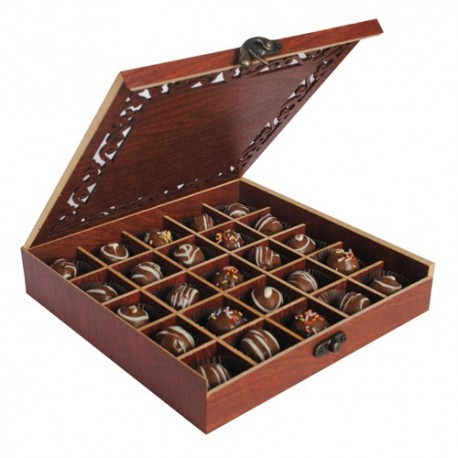
\includegraphics[width=0.5\linewidth]{box-of-chocolate}
	% \caption{Contoh Meriam 1}
\end{figure}

\par\noindent Bocan suka cokelat. Turpa, sebagai fans berat Bocan, memberi hadiah sekotak cokelat berukuran $N \times N$. Tiap cokelat berada pada koordinat $(x,y)$ yang berbeda. Supaya tidak cepat habis, Bocan ingin bermain-main terlebih dahulu dengan cokelatnya.

\par\noindent Bocan melakukan $Q$ aksi. Tiap aksi, ia dapat:

\begin{itemize}
	\item mengambil cokelat di koordinat $(x,y)$.
	\item menaruh cokelat di koordinat $(x,y)$.
	\item menghitung cokelat di segiempat yang kedua ujungnya koordinat $(x_1,y_1)$ dan $(x_2,y_2)$
\end{itemize}

\par\noindent Setiap koordinat di kotak cokelat hanya dapat menampung $1$ buah cokelat.

\subsection*{Format Masukan}

\par\noindent Baris pertama berisi sebuah bilangan bulat $N$ dan $Q$.
\par\noindent $Q$ baris berikutnya berisi salah satu dari:
\begin{itemize}
	\item \lstinline{1 x y}, menaruh cokelat di $(x,y)$
	\item \lstinline{2 x y}, mengambil cokelat di $(x,y)$
	\item \lstinline{3 x1 y1 x2 y2}, menghitung cokelat di segiempat $(x_1,y_1)$ hingga $(x_2,y_2)$
\end{itemize}
\par\noindent Untuk setiap aksi ambil \lstinline{x y}, dijamin ada cokelat di koordinat $(x,y)$. Begitu pula untuk setiap aksi taruh \lstinline{x y}, dijamin tidak ada cokelat di koordinat $(x,y)$.

\subsection*{Format Keluaran}

\par\noindent Untuk tiap query hitung, keluarkan sebuah baris berisi jumlah cokelat di segiempat yang kedua ujungnya $(x_1,y_1)$ dan $(x_2,y_2)$.

\subsection*{Contoh Masukan}

\begin{lstlisting}
10 7
1 1 1
1 2 1
1 3 3
1 6 5
3 1 1 5 4
2 2 1
3 1 1 4 5
\end{lstlisting}

\subsection*{Contoh Keluaran}

\begin{lstlisting}
3
2
\end{lstlisting}

\subsection*{Batasan}

\begin{itemize}
  \item $1 \leq N \leq 10^9$
  \item $1 \leq Q \leq 10^5$
  \item $1 \leq x, y, x_1, y_1, x_2, y_2 \leq N$
  \item $x_1 \leq x_2$ dan $y_1 \leq y_2$
\end{itemize}

\subsection*{Penjelasan}

\par\noindent Sebelum aksi hitung pertama, sudah ada $4$ cokelat, di $(1,1)$, $(2,1)$, dan $(3,3)$, dan $(6,5)$. Tiga cokelat pertama berada di dalam segiempat yang ujungnya $(1,1)$ dan $(5,4)$, sehingga dikeluarkan $3$.

\par\noindent Sebelum aksi hitung kedua, cokelat pada koordinat $(2,1)$ diambil sehingga tersisa $2$ cokelat pada hasil perhitungan.

\par\noindent Sumber gambar:\url{http://www.lazybite.com/82-large_default/signature-wooden-chocolate-box.jpg}

\end{document}
